%(BEGIN_QUESTION)
% Copyright 2011, Tony R. Kuphaldt, released under the Creative Commons Attribution License (v 1.0)
% This means you may do almost anything with this work of mine, so long as you give me proper credit

Dette turbinhastighetsreguleringssystemet ser ikke ut til å regulere riktig. PV i regulatoren er klart lavere enn SP, og har vært det en god stund. Du legger merke til at regulatorutgangen på frontpanelet står på 100\%:

$$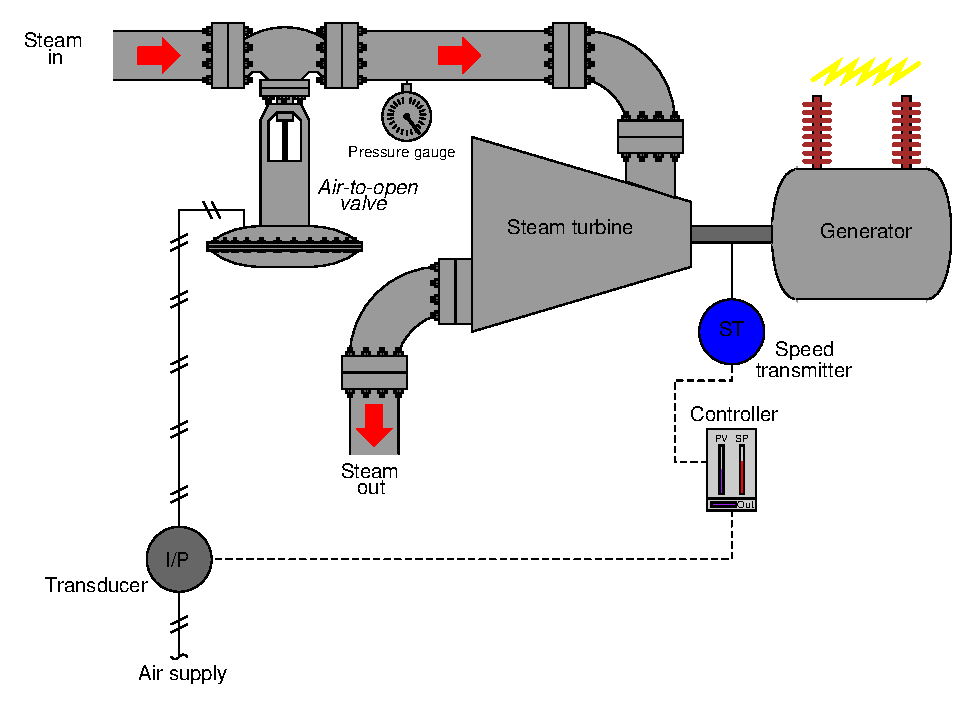
\includegraphics[width=15.5cm]{i00441x01.eps}$$

Første test er å måle sløyfestrømmen i reguleringsventilens (I/P) krets. Multimeteret viser 20.03 mA.

\vskip 10pt

Vurder sannsynligheten for hver oppgitt feil i reguleringssystemet. Vurder én feil om gangen (ingen samtidige feil), og avgjør om hver feil alene kan forklare {\it alle} målinger og symptomer i kretsen.

% No blank lines allowed between lines of an \halign structure!
% I use comments (%) instead, so that TeX doesn't choke.

$$\vbox{\offinterlineskip
\halign{\strut
\vrule \quad\hfil # \ \hfil & 
\vrule \quad\hfil # \ \hfil & 
\vrule \quad\hfil # \ \hfil \vrule \cr
\noalign{\hrule}
%
% First row
{\bf Feil} & {\bf Mulig} & {\bf Umulig} \cr
%
\noalign{\hrule}
%
% Another row
ST ute av kalibrering (gir feil strøm) &  &  \cr
%
\noalign{\hrule}
%
% Another row
SIC-inngang ute av kalibrering (tolker signal feil) &  &  \cr
%
\noalign{\hrule}
%
% Another row
SIC-utgang ute av kalibrering (sender feil mA til I/P) &  &  \cr
%
\noalign{\hrule}
%
% Another row
Trykkmåler ute av kalibrering (viser trykk feil) &  &  \cr
%
\noalign{\hrule}
%
% Another row
I/P ute av kalibrering (gir feil trykk) &  &  \cr
%
\noalign{\hrule}
%
% Another row
Reguleringsventilen er overdimensjonert &  &  \cr
%
\noalign{\hrule}
%
% Another row
Reguleringsventilen er underdimensjonert &  &  \cr
%
\noalign{\hrule}
%
% Another row
SIC er dårlig tunet (tar dårlige reguleringsbeslutninger) &  &  \cr
%
\noalign{\hrule}
%
% Another row
Instrumentluftforsyningen er ikke på fullt trykk &  &  \cr
%
\noalign{\hrule}
} % End of \halign 
}$$ % End of \vbox

\underbar{file i00441}
%(END_QUESTION)





%(BEGIN_ANSWER)

Dette er en vurderingsoppgave, så her gis ingen svar eller hint.

%(END_ANSWER)





%(BEGIN_NOTES)

At regulatorutgangen er mettet høyt samtidig som PV ligger godt under SP betyr at regulatoren forsøker maksimalt å løfte PV opp til SP. Regulatoren tar altså «gode» beslutninger, og PID-algoritmen er neppe feilkilden. Dette er det vi kan si ut fra frontpanelet alene. Deretter må vi sjekke korrespondans i felt mellom PV/Output-visning og faktiske signaler.

\vskip 10pt

Første test viser at regulatoren faktisk sender ut riktig strøm for 100\% Output. Det betyr god korrespondanse mellom Output-visning og reelt utgangssignal. Men vi vet fortsatt ikke om reguleringsventilen faktisk står helt åpen, så feil i I/P, instrumentluft eller ventilen selv er fortsatt mulig.

\vskip 10pt

En annen mulighet, som ofte overses, er feil på målesiden av sløyfen. Vi har ennå ingen data som viser om lav PV i regulatoren samsvarer med virkelig turbinhastighet. Det kan derfor fortsatt være kalibreringsfeil på målesiden: enten i hastighetssenderen eller i regulatorens PV-inngang. Med andre ord kan virkelig turbinhastighet være {\it over} settpunkt, men vises lavt i regulatoren på grunn av feil i målekomponentene.

% No blank lines allowed between lines of an \halign structure!
% I use comments (%) instead, so that TeX doesn't choke.

$$\vbox{\offinterlineskip
\halign{\strut
\vrule \quad\hfil # \ \hfil & 
\vrule \quad\hfil # \ \hfil & 
\vrule \quad\hfil # \ \hfil \vrule \cr
\noalign{\hrule}
%
% First row
{\bf Feil} & {\bf Mulig} & {\bf Umulig} \cr
%
\noalign{\hrule}
%
% Another row
ST ute av kalibrering (gir feil strøm) & $\surd$ &  \cr
%
\noalign{\hrule}
%
% Another row
SIC-inngang ute av kalibrering (tolker signal feil) & $\surd$ &  \cr
%
\noalign{\hrule}
%
% Another row
SIC-utgang ute av kalibrering (sender feil mA til I/P) &  & $\surd$ \cr
%
\noalign{\hrule}
%
% Another row
Trykkmåler ute av kalibrering (viser trykk feil) &  & $\surd$ \cr
%
\noalign{\hrule}
%
% Another row
I/P ute av kalibrering (gir feil trykk) & $\surd$ &  \cr
%
\noalign{\hrule}
%
% Another row
Reguleringsventilen er overdimensjonert &  & $\surd$ \cr
%
\noalign{\hrule}
%
% Another row
Reguleringsventilen er underdimensjonert & $\surd$ &  \cr
%
\noalign{\hrule}
%
% Another row
SIC er dårlig tunet (tar dårlige reguleringsbeslutninger) &  & $\surd$ \cr
%
\noalign{\hrule}
%
% Another row
Instrumentluftforsyningen er ikke på fullt trykk & $\surd$ &  \cr
%
\noalign{\hrule}
} % End of \halign 
}$$ % End of \vbox

%INDEX% Basics, control loop troubleshooting: determining cause of control problem
%INDEX% Process: steam turbine generator

%(END_NOTES)
